\documentclass[
                % aspectratio=169, 
                14pt,
                % notes,
                % notes=only,
                ]{beamer}


\usepackage[utf8]{inputenc}
\usepackage{blindtext}
\usepackage{multicol}
\usepackage{booktabs} % For better-looking tables
\usepackage{caption} % For table captions
\usepackage{siunitx} % For alignment of numbers
\usepackage{pgfplots}
\pgfplotsset{compat=1.18}

%========================================================================
% theme setter
\usetheme[progressbar=frametitle]{Madrid}
% \usetheme[progressbar=frametitle]{metropolis}


%========================================================================
% citing and referencing
%% APA bibliography styles
%%%%%%%%%%%%%%%%%%%%%%%
%% To change the style, put a % in front of the second line of the current style and
%% remove the % from the second line of the style you would like to use.
\usepackage[american]{babel}
\usepackage{csquotes}
\usepackage[style=apa, backend = biber]{biblatex}
\bibliography{ref.bib}


% Required package
\usepackage{tikz}

%========================================================================
% Define Optocase Group colors
\definecolor{optocaseblue}{RGB}{0,102,204}
\definecolor{optocasegray}{RGB}{128,128,128}

% Set colors
\setbeamercolor{structure}{fg=optocaseblue}
\setbeamercolor{title}{fg=optocaseblue}
\setbeamercolor{author}{fg=optocasegray}
\setbeamercolor{date}{fg=optocasegray}

%========================================================================
% Customize title page
\defbeamertemplate*{title page}{customized}[1][]
{
  \vspace{1cm}
  \begin{center}
    \usebeamerfont{title}\inserttitle\par
    \vspace{0.3cm}
    \usebeamerfont{subtitle}\insertsubtitle\par
    \vspace{1cm}
    \usebeamerfont{author}\insertauthor\par
    \vspace{0.2cm}
    \usebeamerfont{institute}\insertinstitute\par
    \vspace{0.2cm}
    \usebeamerfont{date}\insertdate\par
  \end{center}
}
%========================================================================
% Customize frame title
% \setbeamertemplate{frametitle}
% {
%   \vspace{0.5cm}
%   \begin{center}
%     \textbf{\insertframetitle}
%   \end{center}
% }

%========================================================================
% % Add Optocase Group logo to every frame
% \logo{
\includegraphics[width=1.5cm]{images/optocase_logo.png}}

%========================================================================
% Embed logo in background
\setbeamertemplate{background}{
    \begin{tikzpicture}[remember picture,overlay]
        \node[opacity=0.015] at (current page.center) {
\includegraphics[width=8cm]{Figures/optocase_logo.png}};
    \end{tikzpicture}
}


%=================================================================

% for converting to a page slides and handouts
% \usepackage{pgfpages}
% \pgfpagesuselayout{6 on 1}[border shrink=1mm]
% \pgfpageslogicalpageoptions{1}{border code=\pgfsetlinewidth{3pt}\pgfusepath{stroke}}
% \pgfpageslogicalpageoptions{2}{border code=\pgfsetlinewidth{3pt}\pgfusepath{stroke}}
% \pgfpageslogicalpageoptions{3}{border code=\pgfsetlinewidth{3pt}\pgfusepath{stroke}}
% \pgfpageslogicalpageoptions{4}{border code=\pgfsetlinewidth{3pt}\pgfusepath{stroke}}
% \pgfpageslogicalpageoptions{5}{border code=\pgfsetlinewidth{3pt}\pgfusepath{stroke}}
% \pgfpageslogicalpageoptions{6}{border code=\pgfsetlinewidth{3pt}\pgfusepath{stroke}}


%=================================================================
% for notes that can be uused in the presentation in pyumpress
% \usepackage{pgfpages}
% \setbeameroption{show notes}
% \setbeameroption{show notes on second screen=right}


%=================================================================
% Removes navigation symbols
\beamertemplatenavigationsymbolsempty
\setbeamertemplate{navigation symbols}{}


%=================================================================
% Define acronyms
\usepackage{glossaries}

% Define acronyms
\newacronym{svm}{SVM}{Support Vector Machine}
\newacronym{logmar}{LogMAR}{log(MAR)}
\newacronym{ml}{ML}{Machine Learning} % include the acronyms from acro.tex
\renewcommand*{\glstextformat}[1]{\textbf{#1}} % Redefine appearance of acronyms as keywords
\makeglossaries % Generate the glossary


\title{Optometry Case Studies}
\author{Augutsine Musoke Ntaate}
\institute{OptoCase}
\date{\today}

\begin{document}

\begin{frame}
  \titlepage
\end{frame}

\begin{frame}[shrink=20]{Table Of Contents}

    % \footnotesize
    % \scriptsize
    \tiny
    % \small
    \begin{multicols}{2}
    \tableofcontents
    \end{multicols}

\end{frame}


\section{Key Words}

% 2 to 5 key words that identify diagnoses or interventions in this case report, including "case report"

% List of acronyms
\begin{frame}
\frametitle{Key Words}
\printglossary[type=\acronymtype]
\end{frame}

\section{ Abstract (no references)}

\subsection{Introduction: What is unique about this case and what does it add to the scientific literature? (no references)}
\begin{frame}{Abstract}
    \begin{itemize}
        \item water 
        \item Air 
        \item Fire 
        \item Earth 
    \end{itemize}
\end{frame}

\subsection{Main symptoms and/or important clinical findings}


\subsection{The main diagnoses, therapeutic interventions, and outcomes.}


\subsection{Conclusion-What is the main "take-away" lesson(s) from this case?}

\section{Introduction}

\subsection{One or two paragraphs summarizing why this case is unique (may include references)}




\section{Patient Information}

\subsection{De-identified patient specific information.}
\subsection{Primary concerns and symptoms of the patient}
\subsection{Medical, family, and psycho-social history including relevant genetic information Reported on Line}
\subsection{Relevant past interventions with outcomes}

\section{Clinical Findings}
\subsection{Describe significant physical examination (PE) and important clinical findings}

\input{presentationSections/TimeLine/TimeLine}

\section{Diagnostic Assessment}
\subsection{Diagnostic testing (such as PE, laboratory testing, imaging, surveys)}
\subsection{Diagnostic challenges (such as access to testing, financial, or cultural)}
\subsection{Diagnosis (including other diagnoses considered)}
\subsection{Prognosis (such as staging in oncology) where applicable}

\begin{frame}[shrink=35]{Diagnostic Assessment}
    \begin{table}[htbp]
\centering
\caption{Eye Test Results}
\begin{tabular}{|c|c|c|c|}
\hline
\textbf{Date} & \textbf{Visual Acuity} & \textbf{Intraocular Pressure} & \textbf{Remarks} \\ \hline
2022-01-01 & 20/20 & 15 mmHg & Normal \\
2022-04-15 & 20/25 & 16 mmHg & Slight decrease in visual acuity \\
2022-08-20 & 20/30 & 18 mmHg & Further decrease in visual acuity \\
2023-01-10 & 20/40 & 20 mmHg & Significant decrease in visual acuity \\
\hline
\end{tabular}
\end{table}
\end{frame}

\begin{frame}[shrink=20]{Diagnostic Assessment}
    
\begin{table}[htbp]
    \centering
    \caption{Eye Examination Results for Patient X}
    \label{tab:eye_exam_results}
    \begin{tabular}{ll}
        \toprule
        \textbf{Test} & \textbf{Result} \\
        \midrule
        Visual Acuity (VA) & 20/20 \\
        Refraction Powers & -1.00 (-0.50 @ 180) \\
        Intraocular Pressures (IOP) & 15 mmHg (OD), 16 mmHg (OS) \\
        Pupillary Distance (PD) & 62 mm \\
        Slit Lamp Exam & Normal anterior segment \\
        % Add more rows for additional tests
        Gonioscopy & Open angles \\
        Fundoscopy & Clear optic disc, healthy retina \\
        Visual Fields & Full, no defects \\
        Corneal Topography & Regular astigmatism \\
        \bottomrule
    \end{tabular}
\end{table}

\end{frame}

\begin{frame}[shrink=20]{Diagnostic Assessment}
    
\begin{figure}[htbp]
    \centering
    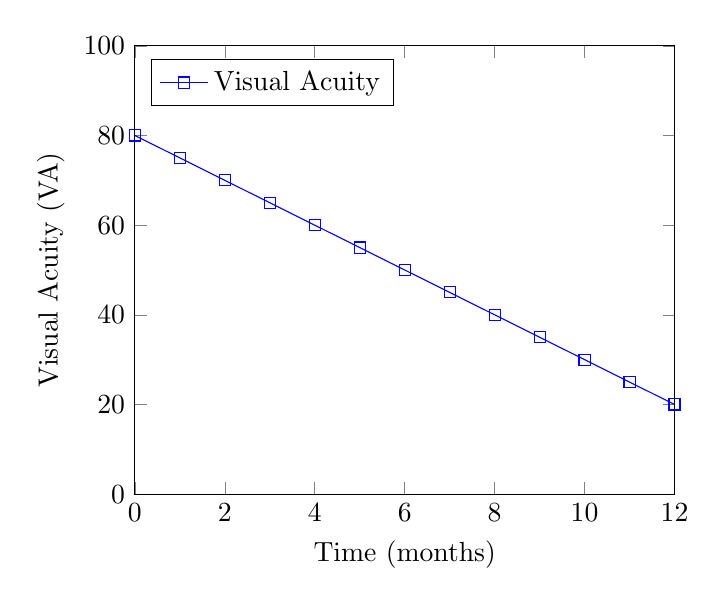
\begin{tikzpicture}
        \begin{axis}[
            xlabel={Time (months)},
            ylabel={Visual Acuity (VA)},
            xmin=0, xmax=12,
            ymin=0, ymax=100,
            xtick={0,2,4,6,8,10,12},
            ytick={0,20,40,60,80,100},
            legend pos=north west,
            grid style=dashed,
        ]
        
        \addplot[
            color=blue,
            mark=square,
        ]
        coordinates {
            (0,80)(1,75)(2,70)(3,65)(4,60)(5,55)(6,50)(7,45)(8,40)(9,35)(10,30)(11,25)(12,20)
        };
        
        \legend{Visual Acuity}
        
        \end{axis}
    \end{tikzpicture}
    \caption{Visual Acuity Over Time}
    \label{fig:va_graph}
\end{figure}
\end{frame}



\section{Therapeutic Intervention}
\subsection{Types of therapeutic intervention (such as pharmacologic, surgical, preventive, self-care)}

\subsection{Administration of therapeutic intervention (such as dosage, strength, duration)}

\subsection{Changes in therapeutic intervention (with rationale)}
\begin{frame}[allowframebreaks]{Changes in therapeutic intervention (with rationale)}
        in the \cite{wajuihian2021gender}

        We will discuss various machine learning algorithms, such as \gls{svm} and \acrshort{ml}.and use of the \acrshort{logmar} is very need in such cases

        \note{The etiology of infantile esotropia is unknown}
        \note[item]{Worth's sensory theory: suggests that there is an irreparable congenital defect 
        in the infant's visual system and that surgery can be carried 
        out at leisure mostly for cosmetic purposes}
        \note[item]{Chavasse's motor theory: motor alignment leads 
        to a poor sensory status, which, if left untreated, leads to strabismus.}
\end{frame}


\section{Follow-up and Outcomes}
\subsection{Clinician and patient-assessed outcomes (if available)}
\subsection{Important follow-up diagnostic and other test results}
\subsection{Intervention adherence and tolerability (How was this assessed?)}
\subsection{Adverse and unanticipated events}


\input{presentationSections/Discussion/discussion}


\section{Patients Perspective}
\subsection{The patient should share their perspective in one to two paragraphs on the treatment(s) they received.}

\section{Informed Consent}
\subsection{Did the patient give informed consent? Please provide if requested.}



\begin{frame}[shrink=60]{References}

    % \footnotesize
    % \scriptsize
    % \tiny
    \printbibliography
    
    % \begin{multicols}{2}
    % \printbibliography
    % \end{multicols}

\end{frame}

\begin{frame}[plain]
    \begin{center}
        {\Huge Thank You!}
        
        \vspace{1cm}
        
        {\LARGE "Success is not final, failure is not fatal: It is the courage to continue that counts."}
        
        \vspace{0.5cm}
        
        {\large -- Winston Churchill}
        
        \vspace{1cm}
        
        {\Large Any Questions?}
    \end{center}
\end{frame}
% Add more presentationSections and subpresentationSections as needed

\end{document}